\section{Descripción detallada de la solución informática desarrollada}

Se ha desarrollado un sistema capaz de extraer información de documentos.
Concretamente, el sistema tiene soporte para documentos en formato \textit{PDF} y para dos tipos de contrato, los
contratos de alquiler de vivienda entre particulares y los contratos de compraventa de vehículo entre particulares.

Para el desarrollo, se ha seguido un conjunto de buenas prácticas como el uso código limpio y de arquitecturas limpias,
lo que facilita que la solución pueda ser extendida para diferentes casos de uso.

El sistema tiene un primer componente, el componente \textit{Generator}, con capacidad para convertir documentos
\textit{PDF} en texto, tal y como se define en el \textbf{Requisito 1} que se definió en la sección~
\ref{sec:objetives} Objetivos.

Aunque en esta implementación se ha utilizado un sistema concreto para la conversión de documentos \textit{PDF}
en texto, el sistema permite incorporar otras implementaciones que realicen la conversión de otros formatos utilizando
otros elementos de infraestructura.

El sistema tiene un segundo componente, el componente \textit{Reader}, capaz de extraer información a partir de la
salida del componente anterior.
Se ha implementado soporte para dos tipos de documentos concretos: contratos de arrendamiento de vivienda entre
particulares (\textbf{Requisito 2}) y contratos de compraventa de vehículos entre particulares (\textbf{Requisito 3}).

Aunque el sistema está diseñado para usarse en modo librería, integrado dentro de otros sistemas, se desarrollaron dos
interfaces.

La interfaz web está desarrollada con un diseño responsivo, lo que significa que se adapta automáticamente al tamaño de
la pantalla del dispositivo en el que se visualiza.

Al arrastrar y soltar un documento sobre el cuadro de diálogo, la web mostrará un mensaje con los datos del documento en
formato \textit{JSON}.
En la figura~\ref{fig:chapter_5.1.web_interface} se puede ver el resultado de ejecutar un contrato de arrendamiento
de vivienda entre particulares.

\begin{figure}[ht]
    \begin{center}
        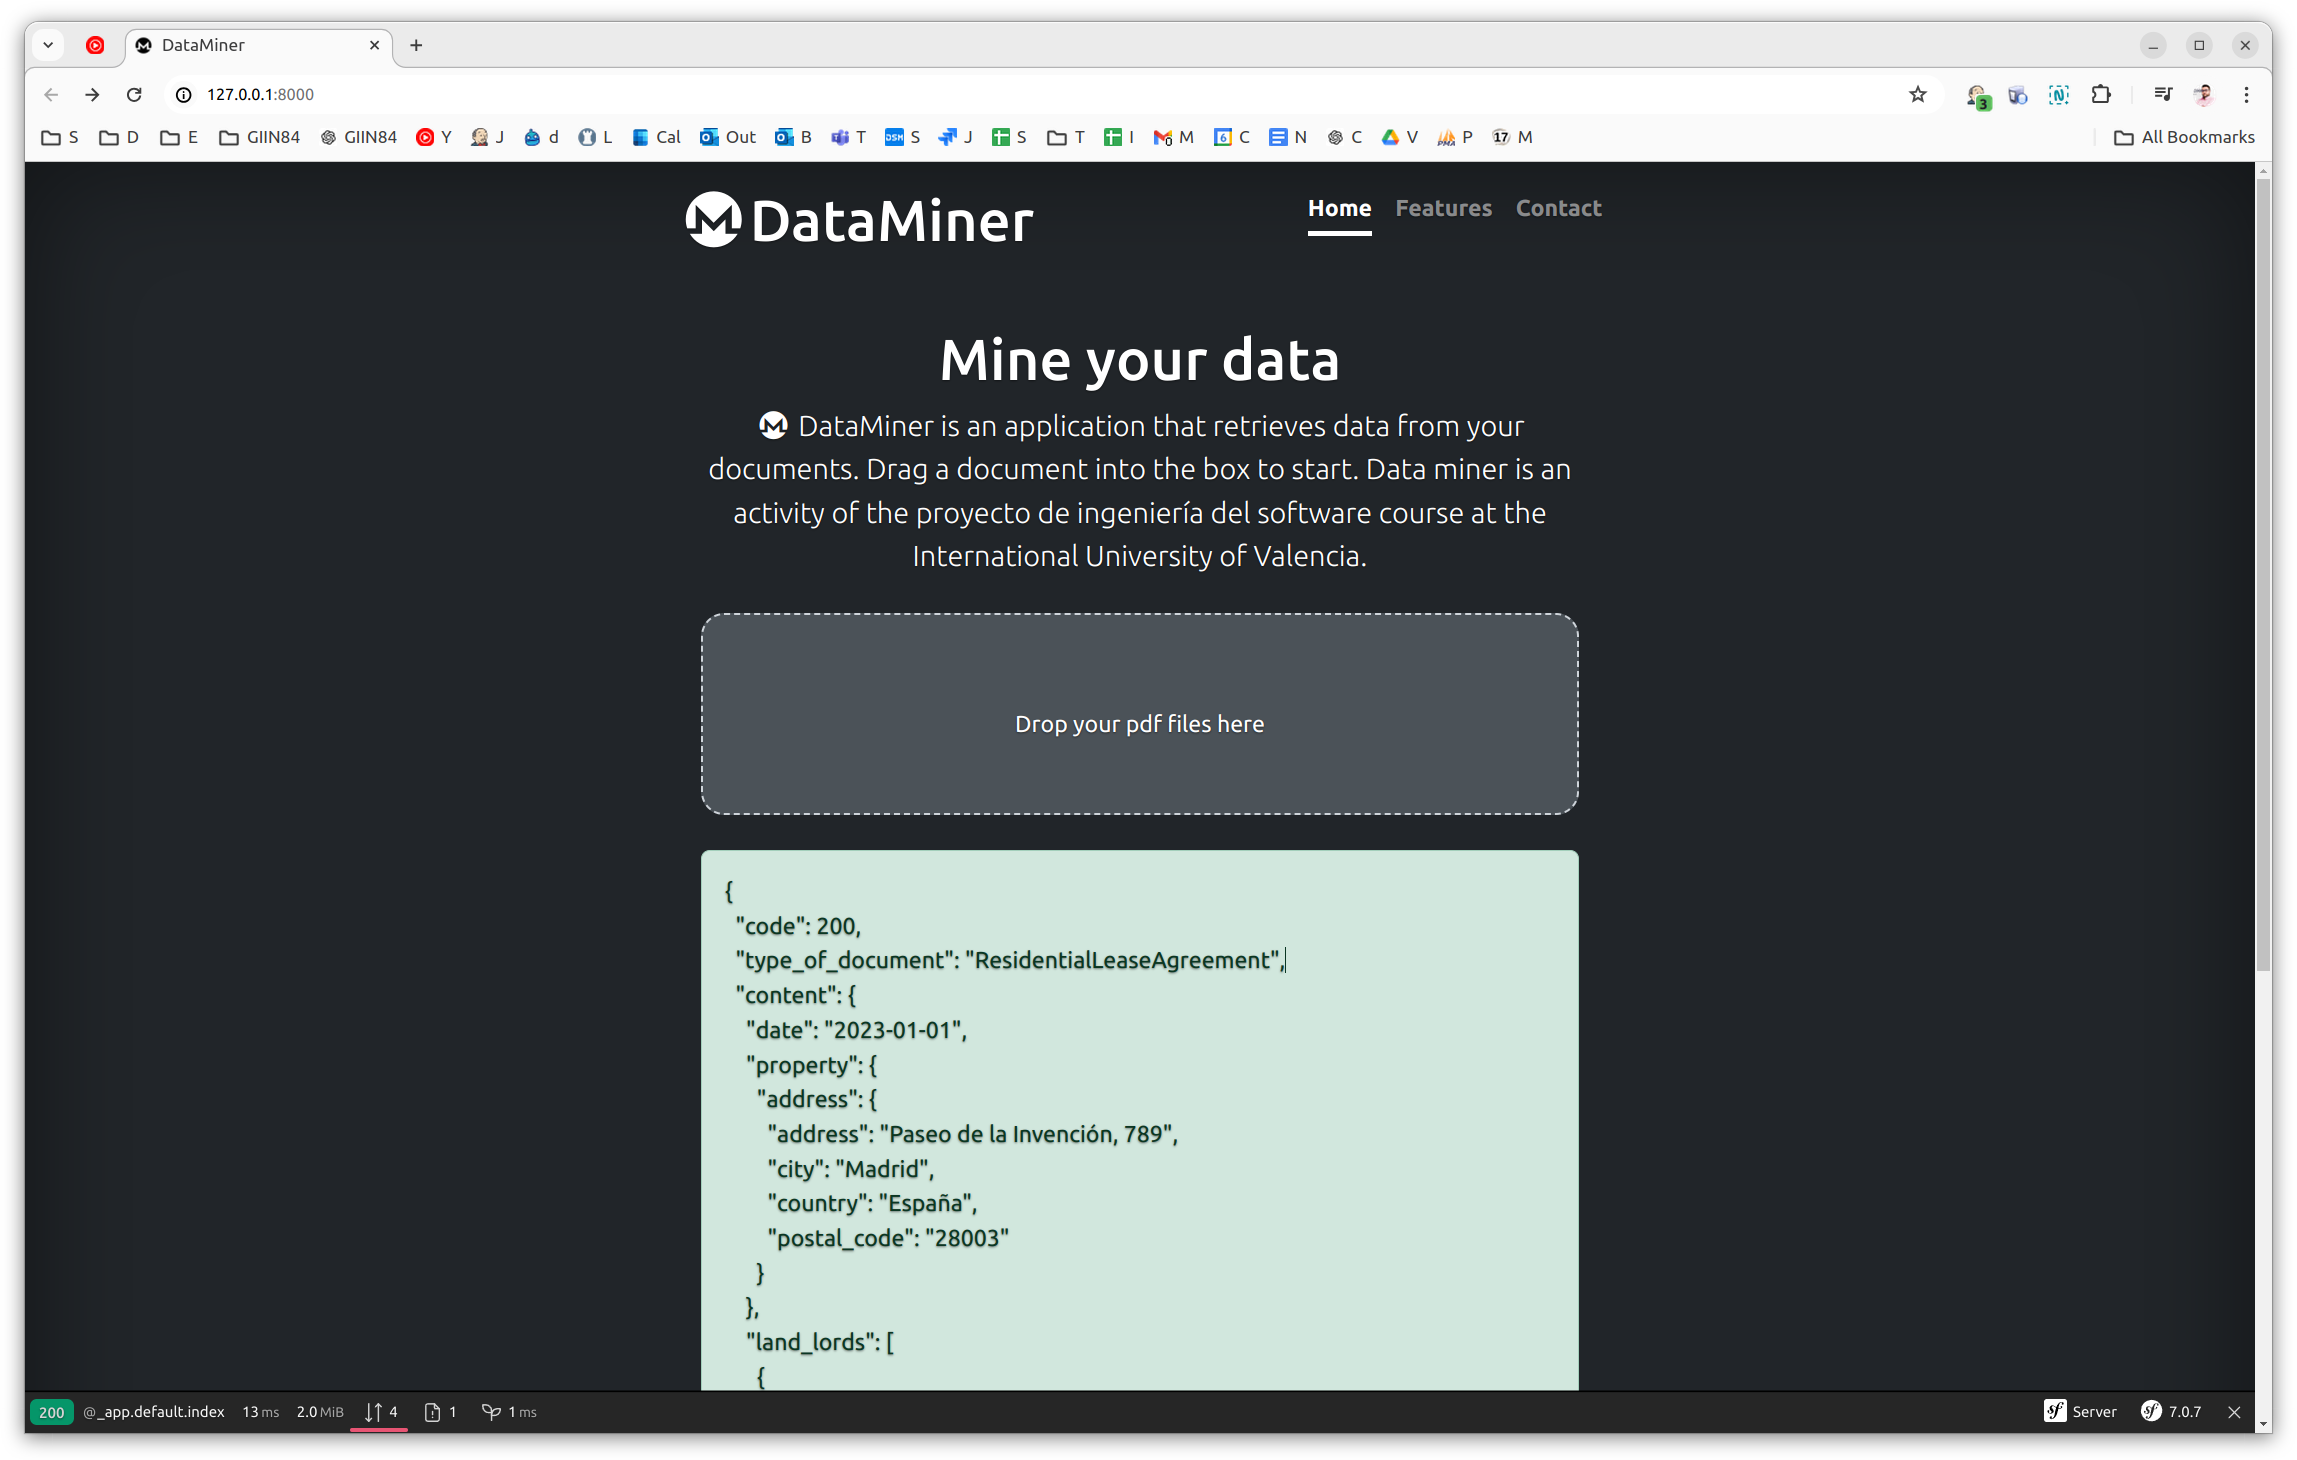
\includegraphics[width=\textwidth]{./chapter/5/images/chapter_5.1.web_interface}
        \caption{Captura del resultado de procesar un documento a través de la interfaz web}
        \label{fig:chapter_5.1.web_interface}
    \end{center}
\end{figure}

La interfaz de línea de comandos está desarrollada de forma que se debe pasar como parámetro la ruta al documento.
En la figura~\ref{fig:chapter_5.1.cli_interface} se puede ver el resultado de ejecutar un contrato de compraventa de
vehículo entre particulares.

\begin{figure}[ht]
    \begin{center}
        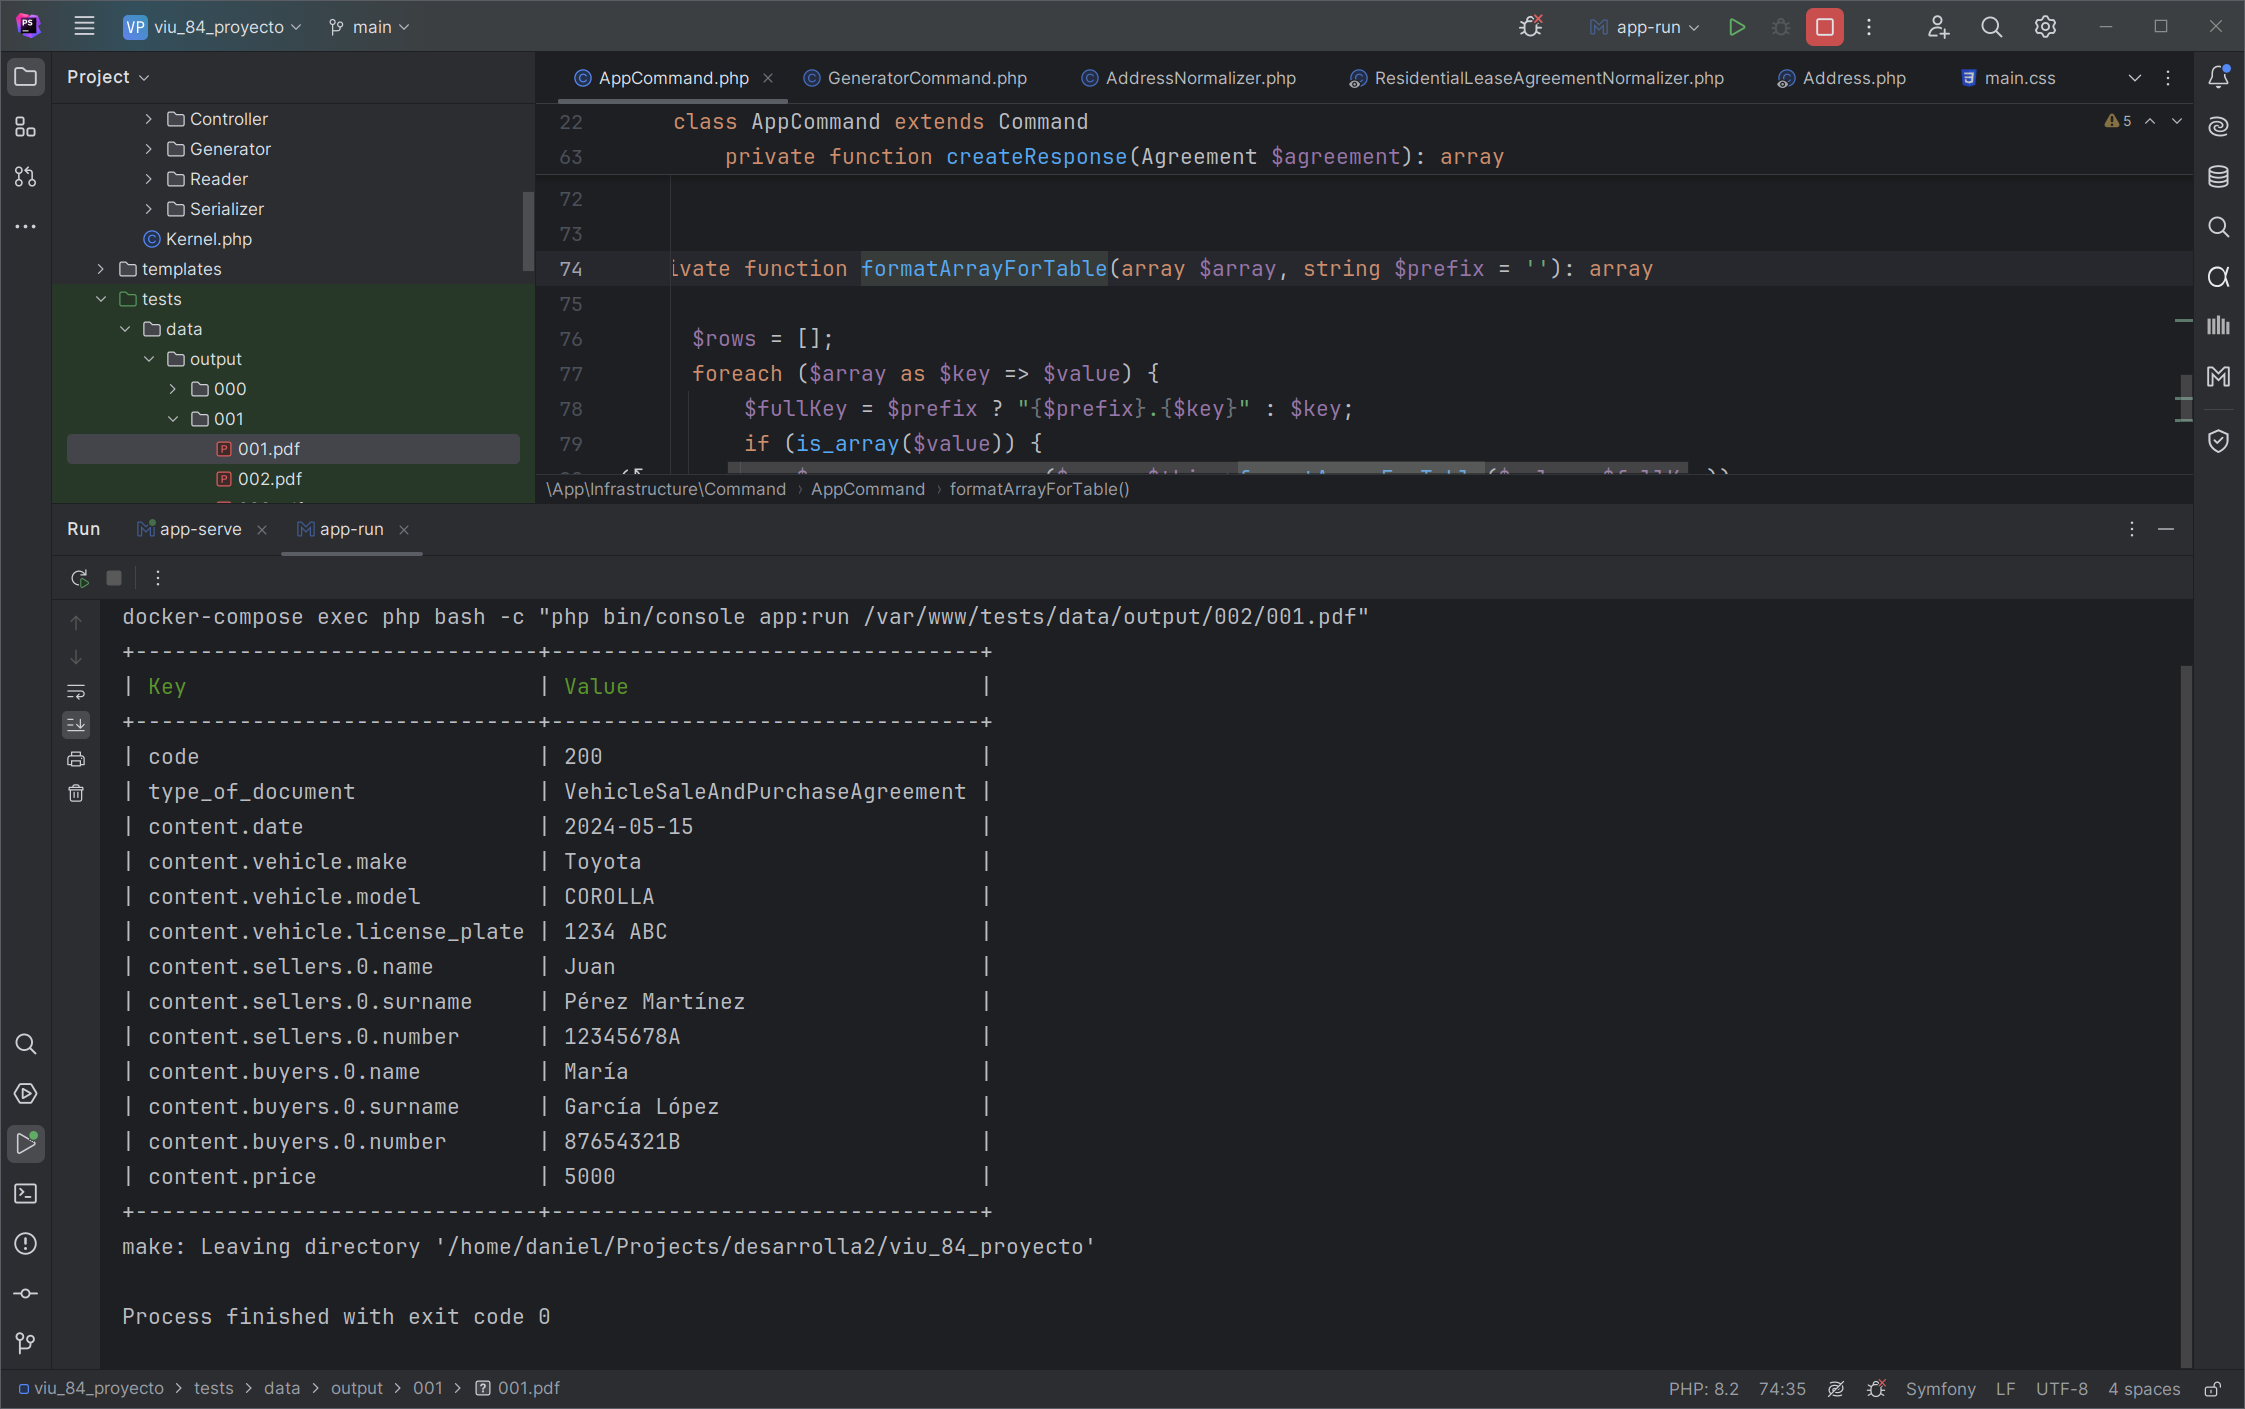
\includegraphics[width=\textwidth]{./chapter/5/images/chapter_5.1.cli_interface}
        \caption{Captura del resultado de procesar un documento a través de la interfaz de línea de comandos}
        \label{fig:chapter_5.1.cli_interface}
    \end{center}
\end{figure}
